\chapter{Rozwiązanie problemu}
\label{chapter-3}

\section{Model rozwiązania}

W pracy zdecydowano się rozwiązać problem na bazie metody opisanej w publikacji \cite{Braun2014}. W tej sekcji zostanie podany zbiór metod użytych do rozwiązanie problemu. Zdefiniowanie i opis poszczególnych metod nastąpi w kolejnych sekcjach rozdziału.

\noindent Przetwarzanie sygnału zaczyna się od obliczenia STFT nagrania wejściowego. Następnie odbywa się przetwarzanie przedstawione na \ref{fig:block_diagram}. Na początku obliczona zostaje macierz widmowej gęstości mocy sygnału (PSD). Następnie za jej pomocą estymowany jest kierunek nadchodzenia fal (DOA). Dzięki połączeniu tych wartości możliwe jest zastosowanie algorytmu automatycznej regulacji głośności (AGC). Ostatnim krokiem jest zastosowanie filtru LCMV, który jako argumenty przyjmuje żądane poziomy wzmocnień, wyestymowane kierunki i sygnał wejściowy. Taki filtr produkuje sygnał wyjściowy. 

\begin{figure}[h]
    \centering
    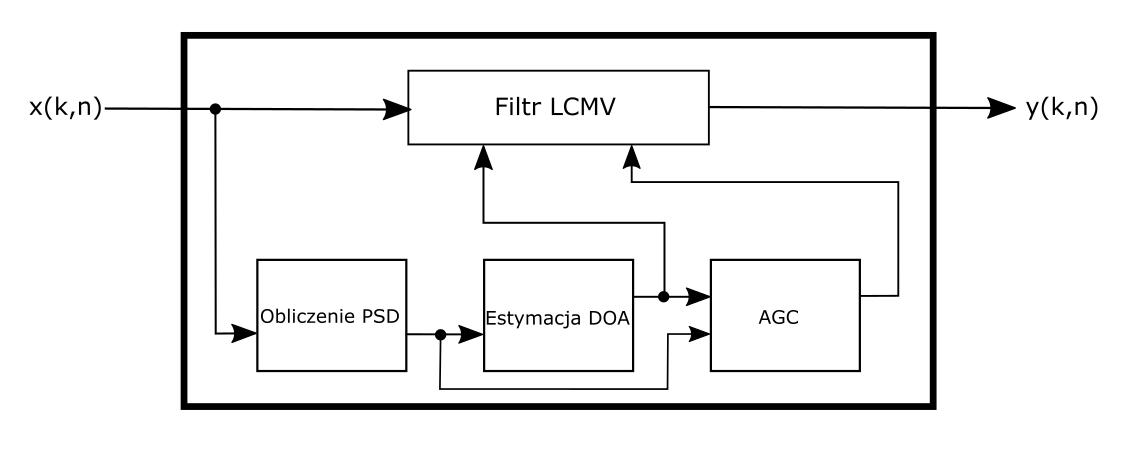
\includegraphics[width=\textwidth]{Images/block_diagram.png}
    \caption{Diagram blokowy}
    \label{fig:block_diagram}
\end{figure}

\section{Widmowa gęstość mocy}

Widmowa gęstość mocy może być zapisana jako:
\begin{equation}
    \label{equation:PSD}
    \phi_{l}(k,n) = \mathrm{E}
    \{|X_{l}(k,n,\bm{\mathrm{d}}_{0})|\}
\end{equation}
Macierz widmowej gęstości mocy definiuje się następująco:

\begin{equation}
    \label{equation:PSD matrix}
    \mathrm{\Phi}(k,n) = \mathrm{E} \, \{\bm{\mathrm{x}}(k,n) \bm{\mathrm{x}}^{H}(k,n)\}
\end{equation}

W praktyce jest obliczana jako średnia z $N$ zebranych próbek:
\begin{equation}
    \label{equation: PSD in practice}
    \mathrm{\Phi}(k,n)=
    \dfrac{1}{N} \sum_{i = n-N}^{n-1}
    \bm{\mathrm{x}}(k,i) \bm{\mathrm{x}}^{H}(k,i)
\end{equation}

Zgodnie z \cite{Thiergart2013}, zakładając, że wszystkie elementy równania \ref{equation:2.2} są nieskorelowane, można zapisać:

\begin{equation}
    \label{equation:PSD signal noise}
    \bm{\mathrm{\Phi}}(k,n) = 
    \sum_{l=1}^{L} \bm{\mathrm{\Phi}}_{l}(k,n) +
    \bm{\mathrm{\Phi}}_{\mathrm{n}}(k,n)
\end{equation}

Gdzie odpowiednio $\bm{\mathrm{\Phi}}_{l}(k,n)$ i $\bm{\mathrm{\Phi}}_{\mathrm{n}}(k,n)$ są macierzami PSD odpowiednio $l$-tej padającej fali i zakłóceń.

\section{Przestrzenna funkcja głośności}

Ważnym elementem systemu będzie sterowanie tak zwaną przestrzenną funkcją głośnośni $G(\theta_{l},n)$. Funkcja ta jest odpowiedzialna za utrzymywanie głośności sygnału wyjściowego na założonym poziomie:

\begin{equation}
    \label{equation:G}
    \mathrm{Y}(k,n)= 
    \sum_{l=1}^{L} G(\theta_{l},n)
    \mathrm{X}_{l}(k,n,\bm{\mathrm{d}}_0)
\end{equation}

\section{Filtr LCMV}

Punktem wyjściowym dla definicji filtru LCMV jest próba zapisania estymaty sygnału wyjściowego $\hat{\mathrm{Y}}(k,n)$ jako:
\begin{equation}
    \label{equation:Y estimation}
    \hat{\mathrm{Y}}(k,n)=
    \bm{\mathrm{w}}^{\mathrm{H}}(k,n)
    \bm{\mathrm{x}}(k,n)
\end{equation}

\noindent Aby znaleźć współncyznniki filtru $\bm{\mathrm{w}}_{\mathrm{n}}(k,n)$, które pozwolą jak najlepiej przybliżyć żądane rozwiązanie należy rozwiązać problem optymalizacyjny zdefiniowany przez dwa poniższe równania:
\begin{equation}
    \label{equation:argmin}
    \bm{\mathrm{w}}_{\mathrm{n}}(k,n) = 
    \underset{\bm{\mathrm{w}}}{\mathrm{arg \, min}} \,
    \bm{\mathrm{w}}^{\mathrm{H}}
    \bm{\mathrm{\Phi}}_{n}
    \bm{\mathrm{w}}
\end{equation}

\begin{equation}
    \label{equation:constraint}
    \bm{\mathrm{w}}^{\mathrm{H}}
    \bm{\mathrm{a}}_{l}(k,n)=
    G(\theta_{l},n),
    \, \, l \in \{1,2,...,L\}
\end{equation}

Ten zapis oznacza, że żądany filtr powinien minimalizować podawane na wejście zakłócenia \ref{equation:argmin} i odpowiednio sterować głośnościami poszczególnych nadchodzących fal \ref{equation:constraint}. Rozwiązanie tak postawionego problemu można znaleźć w \cite{Thiergart2013} zaś wyprowadzenie w \cite{Frost1972}:

\begin{equation}
    \label{equation:lcmv formula}
    \bm{\mathrm{w}}_{\mathrm{n}}=
    \bm{\mathrm{\Phi}}_{n}^{-1}\bm{\mathrm{A}}
    [\bm{\mathrm{A}}^{\mathrm{H}} \bm{\mathrm{\Phi}}_{n} \bm{\mathrm{A}}]^{-1}
    \bm{\mathrm{g}}
\end{equation}

\noindent Gdzie macierz $\bm{\mathrm{A}}(k,n)=
[\bm{\mathrm{a}}_{1}...\bm{\mathrm{a}}_{L}]$ zaś wektor $\bm{\mathrm{g}}(n)=[G(\theta_{1},n)...G(\theta_{L},n)]^{T}$.

\section{Algorytm MUSIC}

MUSIC(ang. Multiple Emitter Location and Signal Parameter Estimation) został opisane w \cite{Schmidt1986}. Nowocześniejsze opracowania można też znaleźć w \cite{DOA} i \cite{Benesty2008} Algorytm pozwala wyestymować kierunki nadchodzenia fali w systemie zawierającym wiele źródeł. Algorytm zakłada przyjęty model sygnału z założeniem, że tło akustyczne to wyłącznie biały szum gaussowski. Obecność innych zakłóceń pogarsza działanie systemu.

\noindent Na potrzeby tej pracy zostanie przedstawiony skrótowo algorytm. Wyprowadzenie znajduje się w wyżej cytowanej publikacji. 
Definiuje się zapis $\bm{\mathrm{a}}(k,n,\theta)$, oznaczający wektor sterującym dla kąta padania $\theta$ i indeksu czasowo-częstotliwościowego $(k,n)$ oraz $\bm{\mathrm{\Phi}}(k,n)$ oznaczający macierz PSD sygnału dla tego samego indeksu czasowo-częstotliwościo

\noindent Liczba nadchodzących fal $L$ może być wyestymowana na przykład zgodnie z publikacją \cite{n_src}. W tej pracy zakłada się jednak, że liczba źródeł jest znana.

\noindent W rozkładzie na wartości własne macierzy $\bm{\mathrm{\Phi}}(k,n)$ wektory własne powiązane z L największymi wartościami własnymi nazywa się wektorami podprzestrzenii sygnału i oznacza jako $\bm{\mathrm{s}}_{i}$, zaś pozostałe wektory- wektorami z podprzestrzenii szumu $\bm{\mathrm{e}}_{i}$. Macierz $\bm{\mathrm{E}}(k,n)$ zawiera w kolejnych kolumnach kolejne wektory podprzestrzenii szumu.

\begin{equation}
    \label{equation:eigenvectors}
    \bm{\mathrm{E}}(k,n)=
    [\bm{\mathrm{e}}_{1}(k,n)...
    \bm{\mathrm{e}}_{M-L}(k,n)]
\end{equation}

\noindent Następnie definiuje się funkcję:
\begin{equation}
    \label{equation:P}
    P(\theta,k,n)=
    \dfrac{1}{
    \bm{\mathrm{a}}^{\mathrm{H}}(\theta,k,n)
    \bm{\mathrm{E}}(k,n)
    \bm{\mathrm{E}}^{\mathrm{H}}(k,n)
    \bm{\mathrm{a}}(\theta,k,n)
    }
\end{equation}
\noindent 
$L$ największych maksimów lokalnych takiej funkcji w dziedzinie kątów uznaje się za wyestymowane kierunki nadchodzenia fali.

\noindent Celem algorytmu jest jednak uzyskanie jednego kierunku nadchodzenia fali dla $n$-tej chwili czasowej. Propozycją autora pracy jest zdefiniować taką funkcję $P_{a}(\theta,n)$, że:
\begin{equation}
    \label{equation:Pa}
    P_{a}(\theta,n) = 
    \dfrac{1}{K}\sum_{k=1}^{K}\,P(\theta,k,n)   
\end{equation}

\noindent Ponownie, $L$ największych maksimów lokalnych wskazuje kierunki nadchodzenia fali.

\newpage
\section{Automatyczna regulacja głośności}

Autor publikacji \cite{Braun2014} proponuje zdefiniowanie funkcji przestrzennego rozkładu głośności(ang. SLD) zapisanego jako:

\begin{equation}
    \label{equation:SLD}
    \Psi(\theta,n)=
    \sum_{k=1}^{K} \beta^{2}(k)
    \sum_{l=1}^{L}\delta_{\theta,\theta_{l}}
    \, \phi_{l}(k,n)
\end{equation}

\noindent Gdzie $(k,n)$ to indeksy czasowo częstotliwościowe, $\delta_{\theta,\theta_{l}}$ to delta Kroneckera- sygnał przyjmujący wartość $1$ dla $\theta_{l}$ i $0$ dla pozostałych.

\noindent Aby wyestymować PSD $\phi_{i}$ $i$-tej fali dokonuje się filtracji filtrem LCMV takim, że:
\begin{equation}
    \label{equation:power estimation}
    \bm{\mathrm{w}}^{\mathrm{H}}\bm{\mathrm{a}}_{l}(k,n)=
    \begin{cases}
        1 \quad l=i \\
        0 \quad l \neq i
    \end{cases}
\end{equation}


\noindent Wartość współczynników $\beta$ może być określona na podstawie istniejących norm, na przykład \cite{coef}. Autor tej pracy iżynierskiej zdecydował jednak przyjąć wartość:

\begin{equation}
    \label{equation:beta}
    \beta(k) = 1, \,\,\,\ k=\{1,2,...,K\}
\end{equation}

\noindent Definiuje się także długoczasową funkcję przestrzennego rozkładu głośności zdefiniowaną jako:

\begin{equation}
    \label{equation:LT_SLD}
    \Psi(\theta,n)=
    \alpha_{LT}\Psi_{LT}(\theta,n-1)
    +(1-\alpha_{LT})\Psi(\theta,n)
\end{equation}

\noindent To działanie ma na celu wygładzenie funkcji w dziedzinie czasu. Głośność sygnału powinna być niewrażliwa na fluktuacje o bardzo dużych częstotliwościach. Taka definicja funkcji jest tożsama z filtracją dolnoprzepustową za pomocą filtra o nieskończonej odpowiedzi impulsowej(IIR).

\noindent Funkcje nie są zależne od składowej częstotliwościowej bo celem pracy jest wzmocnienie amplitudy całego sygnału a nie poszczególnych pasm.

\noindent Przestrzenną funkcje głośności dla danego kąta możnaby otrzymać za pomocą:

\begin{equation}
    \label{equation:sqrt}
    G(\theta,n)=
    \sqrt{\dfrac{\Psi_{target}(\theta)}{
    \Psi_{LT}(\theta,n)}}
\end{equation}

\noindent Należy jednak zauważyć, że tak obliczona funkcja prowadziłaby do silnego wzmocnienia kierunków, w których nie ma sygnału. Co za tym idzie wzmacniane byłoby tłoakustyczne. Kilkustopniowy błąd estymacji kierunku nadchodzenia fali mógłby w praktyce uniemożliwić poprawne działanie systemu. Aby to uniemożliwić definiuje się minimalną moc uznawaną za sygnał $\Psi_{min}(n)$. Obliczona może być jako:

\begin{equation}
    \Psi_{\min}(n)=
    \max({\dfrac{1}{2\pi} \int_{0}^{2\pi} \Psi(\theta,n) \, \mathrm{d}\theta, \, \Psi_{0}})
\end{equation}
Gdzie $\Psi_{0}$ jest pewną ustaloną granicą.

\newpage

\noindent Następnie  dany jest algorytm do obliczenia wygładzonej przestrzennej funkcji głośności $G'(\theta,n)$:


\begin{algorithm}
  \label{alg:gprim}
  \caption{Obliczanie $G'(\theta,n)$}
  \begin{algorithmic}[1]
    \State Zainicjalizuj $G'(\theta,n)$ wartością 1 dla każdego kierunku
    
    \State  Znajdź maksimum globalne funkcji LT-SLD w dziedzinie kąta($\theta_{\max}$) i oblicz przestrzenną funkcją głośności $G(\theta_{max},n)$ za pomocą
    
    \State Wygeneruj okno przestrzenne o określonej szerokości $\Theta$, które ma wzmocnienie $1$ na brzegach i $G(\theta_{max},n)$ w środku.
    
    \State Umieść okno w $\theta_{\max}$ i wyzeruj wartości funkcji LT-SLD w punktach pokrytych przez okno.
    
    \State Kontynnuj krok 2 tak długo aż wszystie punkty funkcji LT-SLFD są poniżej progu $\Psi_{\min}$.
  \end{algorithmic}
\end{algorithm}

\noindent Następnie oblicza się funkcję wygładzającą $\widehat{G}(\theta,n)$:

\begin{equation}
    \label{equation:Ghat}
    \widehat{G}(\theta,n)=
    \alpha_{G}\widehat{G}(\theta,n)
    + (1-\alpha_{G})G'(\theta,n)
\end{equation}


\noindent Funkcja tej operacji jest taka sama jak \ref{equation:LT_SLD}.





